% Options for packages loaded elsewhere
\PassOptionsToPackage{unicode}{hyperref}
\PassOptionsToPackage{hyphens}{url}
\PassOptionsToPackage{dvipsnames,svgnames,x11names}{xcolor}
\documentclass[
  10pt,
]{article}
\usepackage{xcolor}
\usepackage[margin=0.76in]{geometry}
\usepackage{amsmath,amssymb}
\setcounter{secnumdepth}{-\maxdimen} % remove section numbering
\usepackage{iftex}
\ifPDFTeX
  \usepackage[T1]{fontenc}
  \usepackage[utf8]{inputenc}
  \usepackage{textcomp} % provide euro and other symbols
\else % if luatex or xetex
  \usepackage{unicode-math} % this also loads fontspec
  \defaultfontfeatures{Scale=MatchLowercase}
  \defaultfontfeatures[\rmfamily]{Ligatures=TeX,Scale=1}
\fi
\usepackage{lmodern}
\ifPDFTeX\else
  % xetex/luatex font selection
  \setmainfont[]{Cambria}
\fi
% Use upquote if available, for straight quotes in verbatim environments
\IfFileExists{upquote.sty}{\usepackage{upquote}}{}
\IfFileExists{microtype.sty}{% use microtype if available
  \usepackage[]{microtype}
  \UseMicrotypeSet[protrusion]{basicmath} % disable protrusion for tt fonts
}{}
\makeatletter
\@ifundefined{KOMAClassName}{% if non-KOMA class
  \IfFileExists{parskip.sty}{%
    \usepackage{parskip}
  }{% else
    \setlength{\parindent}{0pt}
    \setlength{\parskip}{6pt plus 2pt minus 1pt}}
}{% if KOMA class
  \KOMAoptions{parskip=half}}
\makeatother
\usepackage{longtable,booktabs,array}
\newcounter{none} % for unnumbered tables
\usepackage{calc} % for calculating minipage widths
% Correct order of tables after \paragraph or \subparagraph
\usepackage{etoolbox}
\makeatletter
\patchcmd\longtable{\par}{\if@noskipsec\mbox{}\fi\par}{}{}
\makeatother
% Allow footnotes in longtable head/foot
\IfFileExists{footnotehyper.sty}{\usepackage{footnotehyper}}{\usepackage{footnote}}
\makesavenoteenv{longtable}
\usepackage{graphicx}
\makeatletter
\newsavebox\pandoc@box
\newcommand*\pandocbounded[1]{% scales image to fit in text height/width
  \sbox\pandoc@box{#1}%
  \Gscale@div\@tempa{\textheight}{\dimexpr\ht\pandoc@box+\dp\pandoc@box\relax}%
  \Gscale@div\@tempb{\linewidth}{\wd\pandoc@box}%
  \ifdim\@tempb\p@<\@tempa\p@\let\@tempa\@tempb\fi% select the smaller of both
  \ifdim\@tempa\p@<\p@\scalebox{\@tempa}{\usebox\pandoc@box}%
  \else\usebox{\pandoc@box}%
  \fi%
}
% Set default figure placement to htbp
\def\fps@figure{htbp}
\makeatother
\setlength{\emergencystretch}{3em} % prevent overfull lines
\providecommand{\tightlist}{%
  \setlength{\itemsep}{0pt}\setlength{\parskip}{0pt}}
\usepackage{bookmark}
\IfFileExists{xurl.sty}{\usepackage{xurl}}{} % add URL line breaks if available
\urlstyle{same}
\hypersetup{
  colorlinks=true,
  linkcolor={Maroon},
  filecolor={Maroon},
  citecolor={Blue},
  urlcolor={Blue},
  pdfcreator={LaTeX via pandoc}}

\author{}
\date{}

\usepackage{float}
\usepackage{needspace}
\begin{document}

\section{Eye Sentinel quality scores and defocus
training}\label{eye-sentinel-quality-scores-and-defocus-training}

November 16, 2026 · \href{quality-alignment.zh.md}{Chinese} ·
\href{quality-alignment.en.pdf}{PDF}

Three runs of defocus-only training with matched exposure are complete.
When the number of defocus applications was similar, defocus-only and
mixed training performed similarly on synthetic defocus. Defocus-only
training improved on the unaugmented control in all three seeds. In the
November 13 q--p plots, the distilled quality model scored about 2.4\%
of original images below 0.20. On validation images with paired FTHNet
scores, the teacher and student assigned low scores to similar numbers
of images.

\subsection{How defocus augmentation affects the disease
model}\label{how-defocus-augmentation-affects-the-disease-model}

The original 18 runs across six arms are complete. The new 16.7\%
defocus-only arm adds three training runs, each with 2,400 optimizer
updates and a completed development evaluation. The four arms below use
the same data splits, three seeds, and 65\% sampling quota for the
original sources. In the 50\% mixed arm, illumination, defocus, and
scatter are equally likely when an augmentation is applied. About one in
six training presentations receives defocus. In table order, the average
counts of defocus applications are 0, 6,547, 6,458, and 19,283. Each run
contains about 38,384 image presentations, including repeat draws.
\href{../../../runs/followup_20261115/matched_defocus/status.json}{Training
status}

Checkpoints were selected on 2,046 model-validation images using mean
AUROC across AIROGS, ODIR, Kaggle, LAG, and KEH. The table averages the
results for the selected checkpoint in each of the three seeds. The
original rule-development set contains 2,053 images, with 814 positives
and 1,239 negatives. Both synthetic conditions use the same 384
development images, including 146 positives. AUROC measures how well the
model ranks positives above negatives.

{\def\LTcaptype{none} % do not increment counter
\Needspace{11\baselineskip}
\begin{longtable}[]{@{}
  >{\raggedright\arraybackslash}p{(\linewidth - 8\tabcolsep) * \real{0.2593}}
  >{\raggedleft\arraybackslash}p{(\linewidth - 8\tabcolsep) * \real{0.2099}}
  >{\raggedleft\arraybackslash}p{(\linewidth - 8\tabcolsep) * \real{0.2099}}
  >{\raggedleft\arraybackslash}p{(\linewidth - 8\tabcolsep) * \real{0.1481}}
  >{\raggedleft\arraybackslash}p{(\linewidth - 8\tabcolsep) * \real{0.1728}}@{}}
\toprule\noalign{}
\begin{minipage}[b]{\linewidth}\raggedright
Training arm
\end{minipage} & \begin{minipage}[b]{\linewidth}\raggedleft
Five-source validation mean
\end{minipage} & \begin{minipage}[b]{\linewidth}\raggedleft
Development originals
\end{minipage} & \begin{minipage}[b]{\linewidth}\raggedleft
Synthetic defocus
\end{minipage} & \begin{minipage}[b]{\linewidth}\raggedleft
Synthetic underexposure
\end{minipage} \\
\midrule\noalign{}
\endhead
\bottomrule\noalign{}
\endlastfoot
No degradation & 0.9608 & 0.9759 & 0.9272 & 0.9727 \\
50\% mixed & 0.9634 & 0.9747 & 0.9593 & 0.9756 \\
16.7\% defocus only & 0.9635 & 0.9727 & 0.9628 & 0.9741 \\
50\% defocus only & 0.9623 & 0.9742 & 0.9676 & 0.9720 \\
\end{longtable}
}

\textbf{Applying defocus about one sixth of the time gives results close
to mixed augmentation on synthetic defocus.} The 16.7\% defocus-only arm
improved over the unaugmented control by 0.0356, with gains of +0.0547,
+0.0354, and +0.0167 across the three seeds. The 95\% case-sampling
interval was {[}+0.0222, +0.0506{]}. The same arm was 0.0035 above mixed
augmentation, with an interval of {[}−0.0028, +0.0097{]}. The intervals
come from 2,000 paired resamples of linked case groups with the training
seeds held fixed.

\textbf{Applying defocus more often brings a smaller additional gain.}
At the common endpoint of 2,400 updates, the unaugmented, 16.7\%
defocus-only, and 50\% defocus-only arms reached 0.9289, 0.9659, and
0.9724 on synthetic defocus. The first increase adds about 6,458 defocus
applications and raises AUROC by 0.0371. The next adds about 12,825
applications and raises AUROC by 0.0064, with gains in all three seeds.
Using the validation-selected checkpoints, the 50\% arm averaged 0.0048
above the 16.7\% arm, with a case-sampling interval that includes zero.
These comparisons inform the choice of augmentation intensity in the
next round. \href{completed-matched-defocus.json}{Per-seed results and
paired intervals}

\textbf{Original, underexposed, and real poor-quality images show where
the gains apply.} On originals, the selected 16.7\% defocus model
averaged 0.0032 below the unaugmented control, with the same direction
in all three seeds. At 2,400 updates, the difference narrowed to −0.0015
and its case-sampling interval included zero. At the 0.5 decision
threshold, selected weights from the 16.7\% arm averaged 74.0 misses and
109.3 false positives, compared with 83.3 and 88.3 for the unaugmented
arm. The four arms performed similarly on underexposed images. All
detected the same 12 human-rated poor-quality positives, which came from
12 linked groups. This human-rated subset contains zero negatives. The
clearest training gain is improved performance under synthetic defocus.

\newpage
\subsection{Low scores from the FTHNet teacher and
student}\label{low-scores-from-the-fthnet-teacher-and-student}

The vertical axis in the November 13 q--p figures is the distilled
quality model's continuous score \(q\). A higher score indicates better
predicted overall image quality. Both development sets use original
images. The independent test is scheduled after model and evaluation
choices are fixed. \href{../2026-11-13/progress-overview.en.md}{q--p
figures and data description}

{\def\LTcaptype{none} % do not increment counter
\Needspace{11\baselineskip}
\begin{longtable}[]{@{}lrrr@{}}
\toprule\noalign{}
Dataset & Images & \(q<0.20\) & \(q<0.10\) \\
\midrule\noalign{}
\endhead
\bottomrule\noalign{}
\endlastfoot
Rule development & 2,053 & 49 (2.39\%) & 9 \\
Model validation & 2,046 & 50 (2.44\%) & 12 \\
\end{longtable}
}

Of the 49 low scores in rule development, 46 come from AIROGS, ODIR, and
Kaggle. The low-score rate is 46/1,220 (3.77\%) in those sources and
3/833 (0.36\%) in the other sources. There are 26 positives and 23
negatives in the low-score group. At the 0.5 decision threshold, the
selected 16.7\% defocus models missed 0, 2, and 1 positives and produced
1, 1, and 3 false positives across the three seeds. These results mostly
describe a small set of low-scoring originals from the three original
sources.

File hashes matched the archived teacher and student scores for 1,188
model-validation images from the three original sources. FTHNet assigned
scores below 0.20 to 41 images (3.45\%), and the student did so for 44
(3.70\%). The two scores fell below 0.20 together for 39 images, with
two below the cutoff only for the teacher and five only for the student.
The median absolute difference was 0.019. Low scores were already
uncommon in the teacher output, and the student retained 39 of the
teacher's 41 low scores. Paired scores from the added sources would show
how that comparison varies by source.
\href{completed-matched-defocus.json}{Paired score counts} ·
\href{../../../data/audit/session_20261110/selected_validation/quality_student/validation_predictions.csv}{Archived
teacher and student scores}

The cutoff \(q<0.20\) identifies one range of the model score. Among 120
real same-eye pairs from Real Fundus, the student consistently gave the
better photo a higher score, while just four of the poorer photos fell
below 0.20. Pairwise ranking and low-score frequency describe different
properties of the score. For glaucoma, the visibility of the disc and
cup also determines how much information is available for
interpretation. \href{quality-inventories.json}{Quality inventories}

\subsection{Degradation strength and the quality
score}\label{degradation-strength-and-the-quality-score}

The paired experiment used 12 images per disease class from each of five
main development sources. The 120 photos come from distinct linked
groups. Each photo received each of the listed degradations. The
baseline used the disease model's padding and 320-pixel resize, followed
by resampling to the quality model's input size. Strong defocus used
Gaussian sigma 5 at a reference field diameter of 512 pixels. Strong
underexposure multiplied brightness by 0.40. Misses use the 60 positive
images and a decision threshold of 0.5.

{\def\LTcaptype{none} % do not increment counter
\Needspace{11\baselineskip}
\begin{longtable}[]{@{}
  >{\raggedright\arraybackslash}p{(\linewidth - 6\tabcolsep) * \real{0.4000}}
  >{\raggedleft\arraybackslash}p{(\linewidth - 6\tabcolsep) * \real{0.2000}}
  >{\raggedleft\arraybackslash}p{(\linewidth - 6\tabcolsep) * \real{0.2615}}
  >{\raggedleft\arraybackslash}p{(\linewidth - 6\tabcolsep) * \real{0.1385}}@{}}
\toprule\noalign{}
\begin{minipage}[b]{\linewidth}\raggedright
Condition, 120 images per row
\end{minipage} & \begin{minipage}[b]{\linewidth}\raggedleft
Median change in \(q\)
\end{minipage} & \begin{minipage}[b]{\linewidth}\raggedleft
Newly below 0.20
\end{minipage} & \begin{minipage}[b]{\linewidth}\raggedleft
Misses
\end{minipage} \\
\midrule\noalign{}
\endhead
\bottomrule\noalign{}
\endlastfoot
320 px baseline & 0.000 & 0 & 6 \\
Mild illumination & −0.026 & 2 & 6 \\
Mild defocus & −0.022 & 1 & 9 \\
Mild scatter & −0.018 & 2 & 5 \\
Strong defocus & −0.323 & 105 & 26 \\
Strong underexposure & −0.218 & 26 & 9 \\
Strong combined & −0.358 & 111 & 24 \\
\end{longtable}
}

\newpage
\begin{figure}[H]
\centering
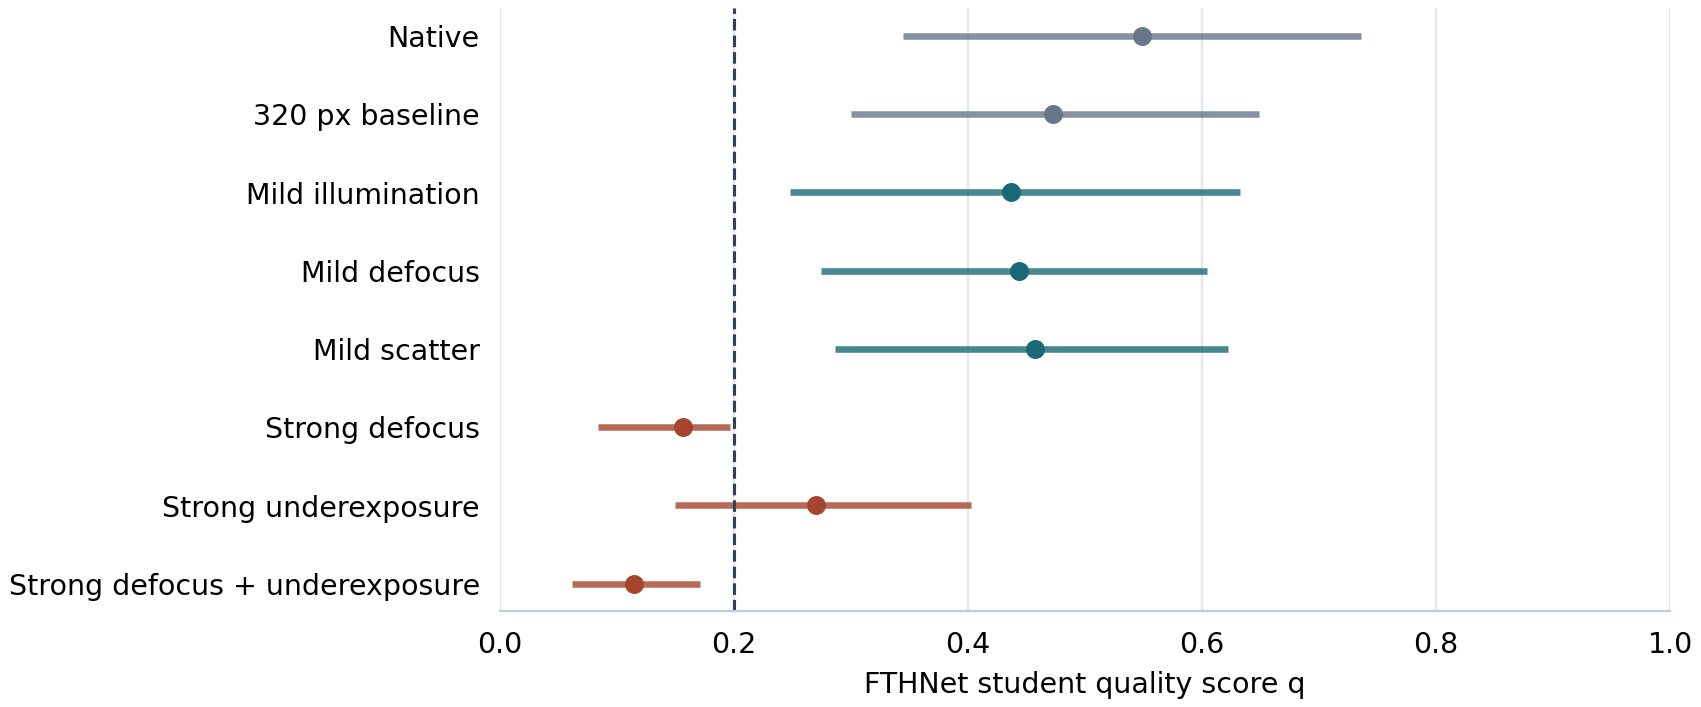
\includegraphics[width=0.95\linewidth,height=\textheight,keepaspectratio,alt={Quality score distributions by degradation condition}]{paired-quality.en.png}
\caption{Quality score distributions by degradation condition}
\end{figure}

Dots mark medians, bars span the 10th to 90th percentiles, and the
dashed line marks \(q=0.20\). Padding and resampling via 320 pixels
shifted the median paired score by −0.058, more than any mild
augmentation. With common preprocessing, each mild condition added just
one or two images below 0.20. Strong defocus populated the low-score
range and reduced disease AUROC from 0.974 to 0.907. Both measurements
inform the choice of severity by showing low-score coverage and the
change in disease discrimination.
\href{paired-summary.json}{Per-condition results}

\subsection{Implications for the next
experiments}\label{implications-for-the-next-experiments}

\textbf{Expand coverage with real poor-quality originals.} The training
set has 72 positive and three negative photos rated poor by human
graders. Rule development has 12 positives. Prioritize real poor-quality
negatives with an independent diagnosis, then enrich positives by source
and device. The local worklist already has 54 low-score photos and 30
controls drawn from 682 prescreened AIROGS NRG candidates. NRG denotes
non-referral. To add clinically confirmed negatives, retain
first-attempt failures and retakes from the same screening workflow,
verify disease status against an independent same-eye reference, and
keep associated photos in the same split.
\href{../../../runs/quality_alignment_20261116/airogs_blinded_quality_review.csv}{Local
candidate list} · \href{https://arxiv.org/html/2302.01738}{AIROGS paper}

\textbf{Set augmentation severity using real images.} Use same-eye
retakes to establish realistic ranges for defocus, underexposure, and
local occlusion, and document whether the disc and cup remain
interpretable. Compare clean and degraded versions with common
preprocessing and report quality scores, gradability, and disease
metrics together. Use moderate variants with preserved diagnostic
structures for disease training, then evaluate original, real
poor-quality, and synthetic images separately. This comparison connects
the observed defocus robustness to the quality measurements in the
proposal. \href{../../../proposal-1106.pdf}{Project proposal}

\href{../../../tools/analyze_matched_defocus_20261116.py}{Analysis
script} · \href{../../../tools/run_matched_defocus_20261116.py}{Training
entry point} · \href{completed-matched-defocus.json}{Results and input
hashes}

\end{document}
